% Paper 2 -- PINN Navier-Stokes refinement of HIAD aerothermal fields (IEEE)
\documentclass[conference]{IEEEtran}
\IEEEoverridecommandlockouts
\usepackage[T1]{fontenc}
\usepackage[utf8]{inputenc}
\usepackage{amsmath,amssymb}
\usepackage{graphicx}
\usepackage{booktabs}
\usepackage{hyperref}
\usepackage{cite}
\graphicspath{{figures/}}

\begin{document}

\title{Physics-Informed Neural Network Refinement of Navier-Stokes Aerothermal Fields on a Hypersonic Inflatable Decelerator}

\author{
\IEEEauthorblockN{Wahyu Suryo Samudro}
\IEEEauthorblockA{Magister Program in Aerospace Engineering\\
Institut Teknologi Bandung, Bandung, Indonesia\\
Correspondence: albertstarfield@protonmail.com}
}

\maketitle

\noindent\textbf{Abstract.}\quad
This paper presents a Physics-Informed Neural Network (PINN) that refines the aerothermal fields produced by Direct Simulation Monte Carlo on a hypersonic inflatable aerodynamic decelerator. The governing equations retained for regularization are the compressible Navier-Stokes equations, treated as a continuum regularization layer whose residuals are informative only where the cell-scale Knudsen number remains inside the continuum band. The network loss combines residual terms on the continuity, momentum and energy equations, data mismatch against the DSMC surface quantities, and Kriging denoising of the DSMC scatter. A two-stage training protocol, automatic differentiation for PDE residuals, and normalization/scaling schedules are used. The refined fields support only the survivability comparison, since the PINN preserves continuum behavior. For the active five-ply Gen-2 stack, the refined-flux survivability comparison gives a backface temperature of $955.66~\mathrm{K}$, exceeding both the $773~\mathrm{K}$ Kapton limit and the $523.15~\mathrm{K}$ IRVE-3 structural limit (companion TPS paper). The contribution is a reproducible PINN pipeline embedded in the StellarOrion software stack.
\par\vspace{0.5em}

\noindent\textit{Keywords:}\quad
PINN, Navier-Stokes, DSMC, HIAD, Aerothermodynamics, Kriging, Machine Learning in CFD
\par\vspace{1em}

\section{Introduction}
Continuum fields are needed for the aerothermal design even when the upstream solution is rarefied, because thermal-protection-system response is continuum-driven. A PINN provides a differentiable, dense reconstruction of velocities, pressures and temperatures from the sparse DSMC samples while penalizing PDE residuals. This paper documents the PINN thread of the StellarOrion framework. The objectives are to present the architecture, the composite loss, the denoising step, and the training protocol, and to state the limits of the continuum assumption.

\section{Governing Equations}
The compressible Navier-Stokes equations in conservative form are used as the PDE residual source, including the continuity, momentum and energy equations. Automatic differentiation supplies the partial derivatives of the network output with respect to spatial and temporal coordinates. Figure~\ref{fig:gov} shows the retained equation set.

\begin{figure}[t]
\centering
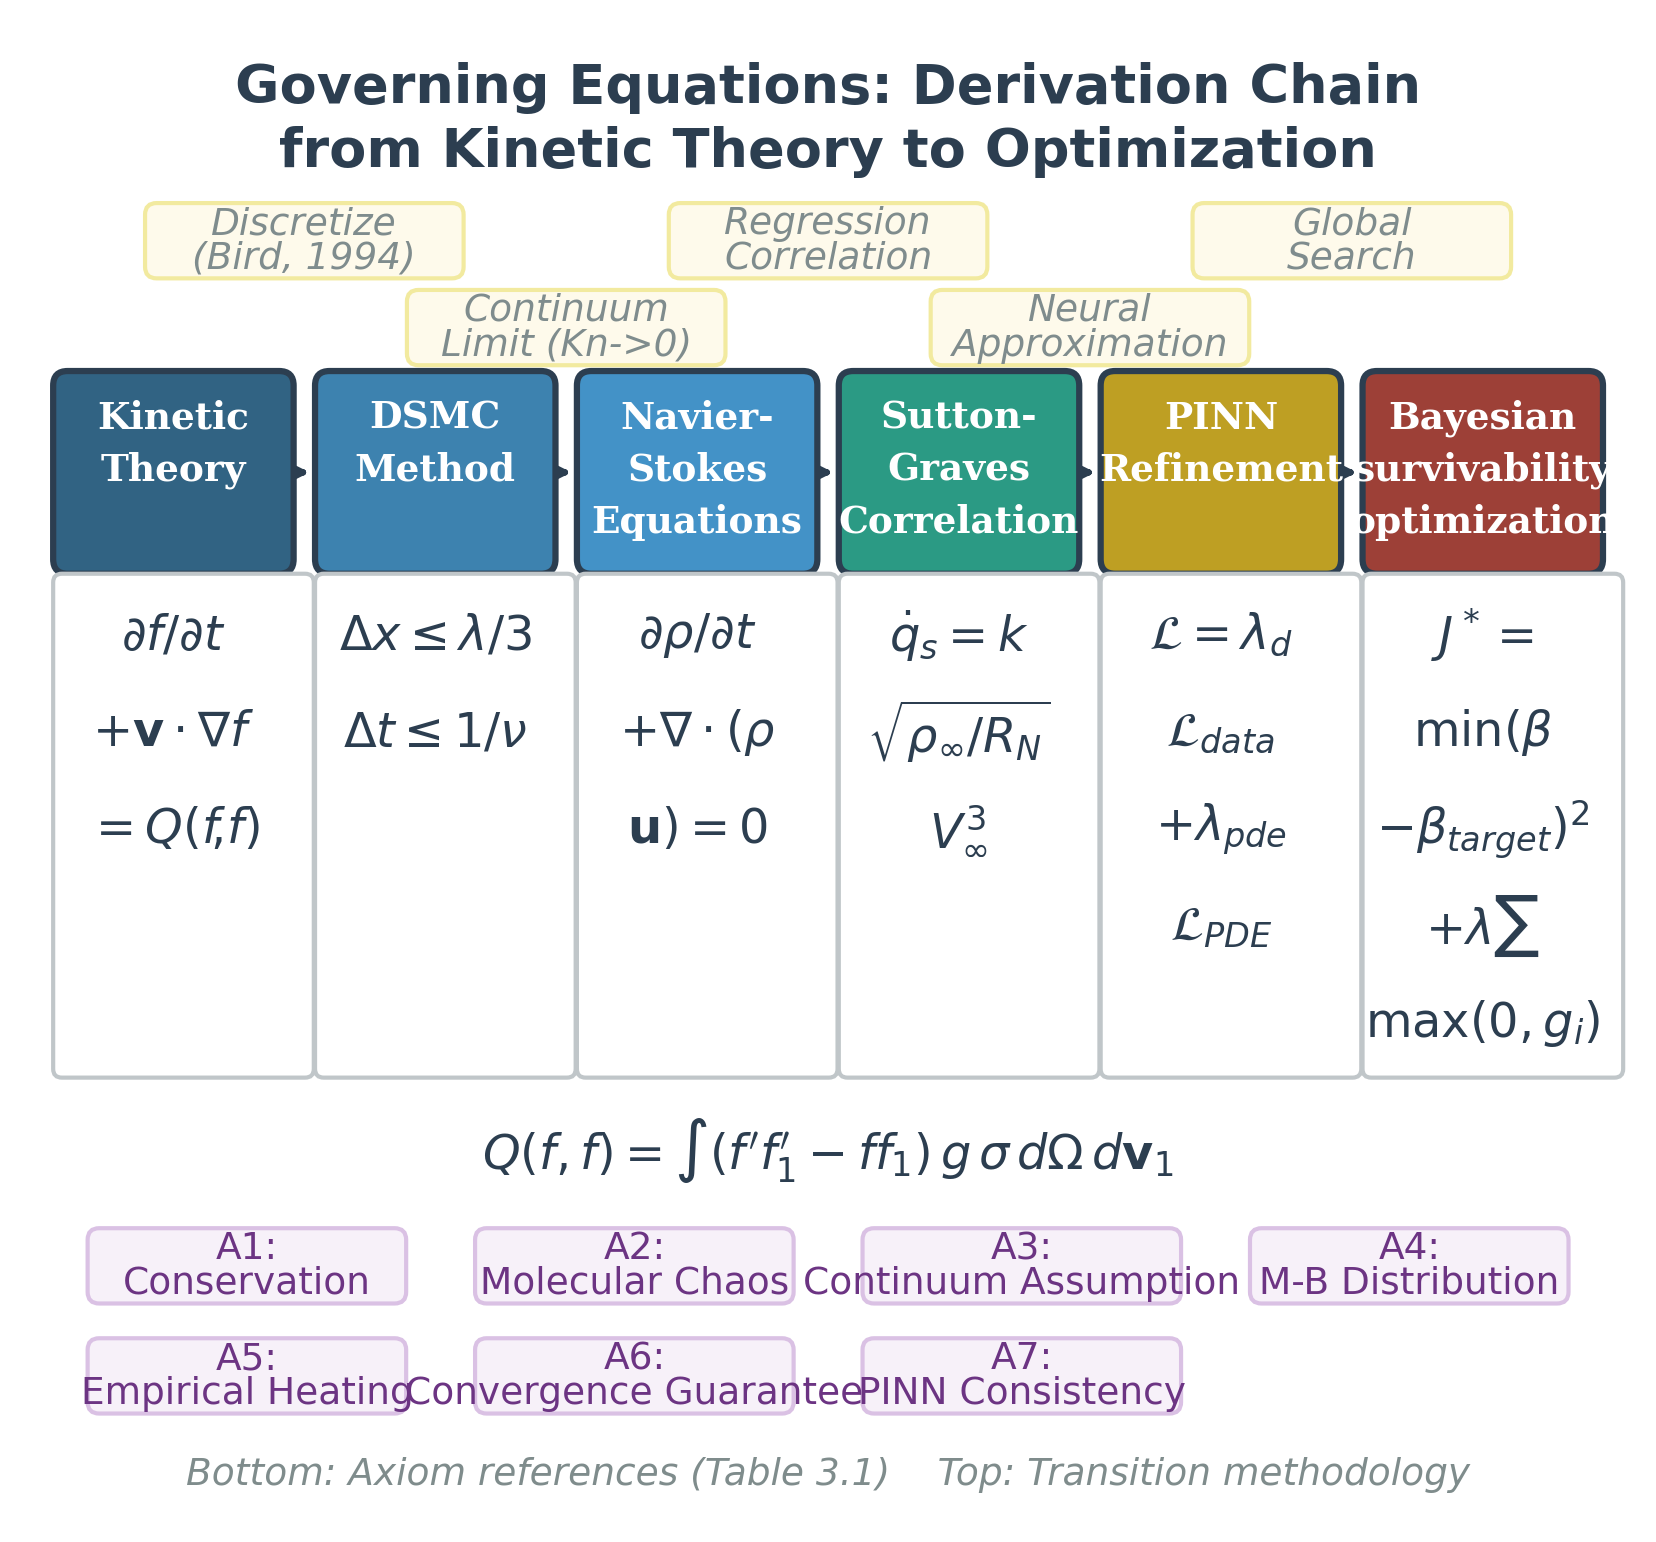
\includegraphics[width=0.9\columnwidth]{governing_equations.png}
\caption{Compressible Navier-Stokes equations retained for PINN regularization.}
\label{fig:gov}
\end{figure}

\section{Network Architecture}
The network is a fully connected surrogate whose input consists of the spatial coordinates and a freestream-condition vector, and whose output consists of velocity, pressure and temperature fields. A separate Kriging denoiser smooths the DSMC scatter before the data term is evaluated. The architecture is shown in Fig.~\ref{fig:arch}.

\begin{figure}[t]
\centering
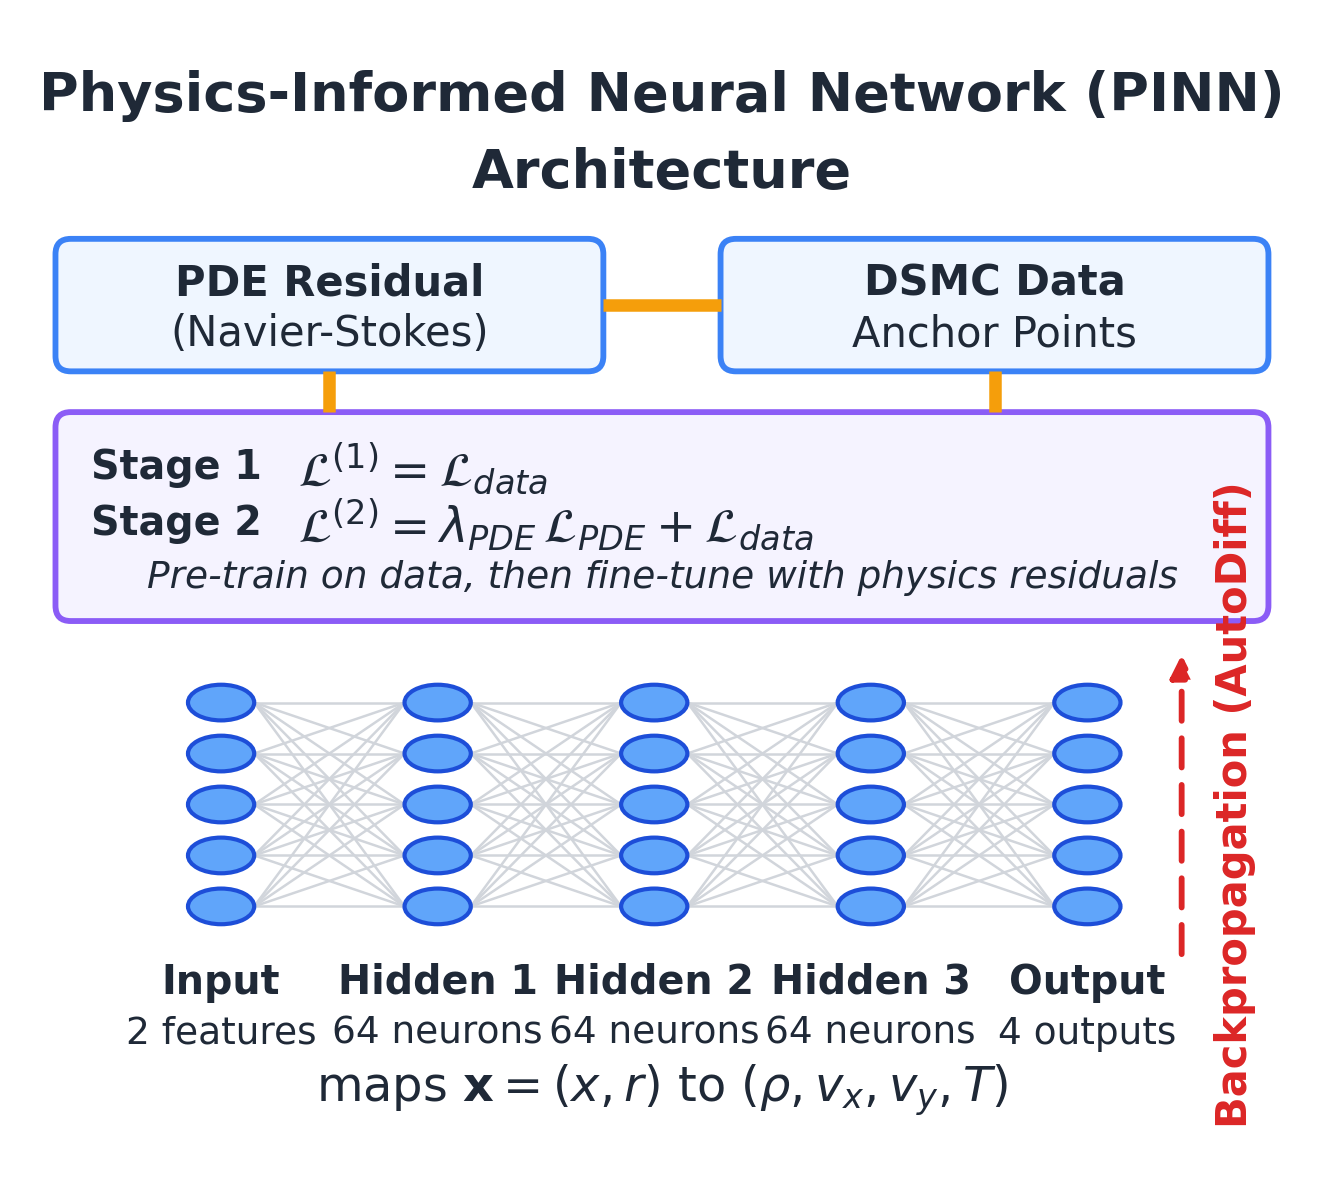
\includegraphics[width=0.9\columnwidth]{pinn_architecture.png}
\caption{PINN architecture with a Kriging denoising pre-stage.}
\label{fig:arch}
\end{figure}

\section{Composite Loss}
The loss is the sum of a PDE residual term, a data-mismatch term against the DSMC surface and near-body quantities, and a Kriging-denoised smoothness penalty. The PDE residual term enforces the Navier-Stokes equations; the data term anchors the solution to the DSMC results. Training follows a two-stage protocol. Figure~\ref{fig:conv} shows the convergence of residuals.

\begin{figure}[t]
\centering
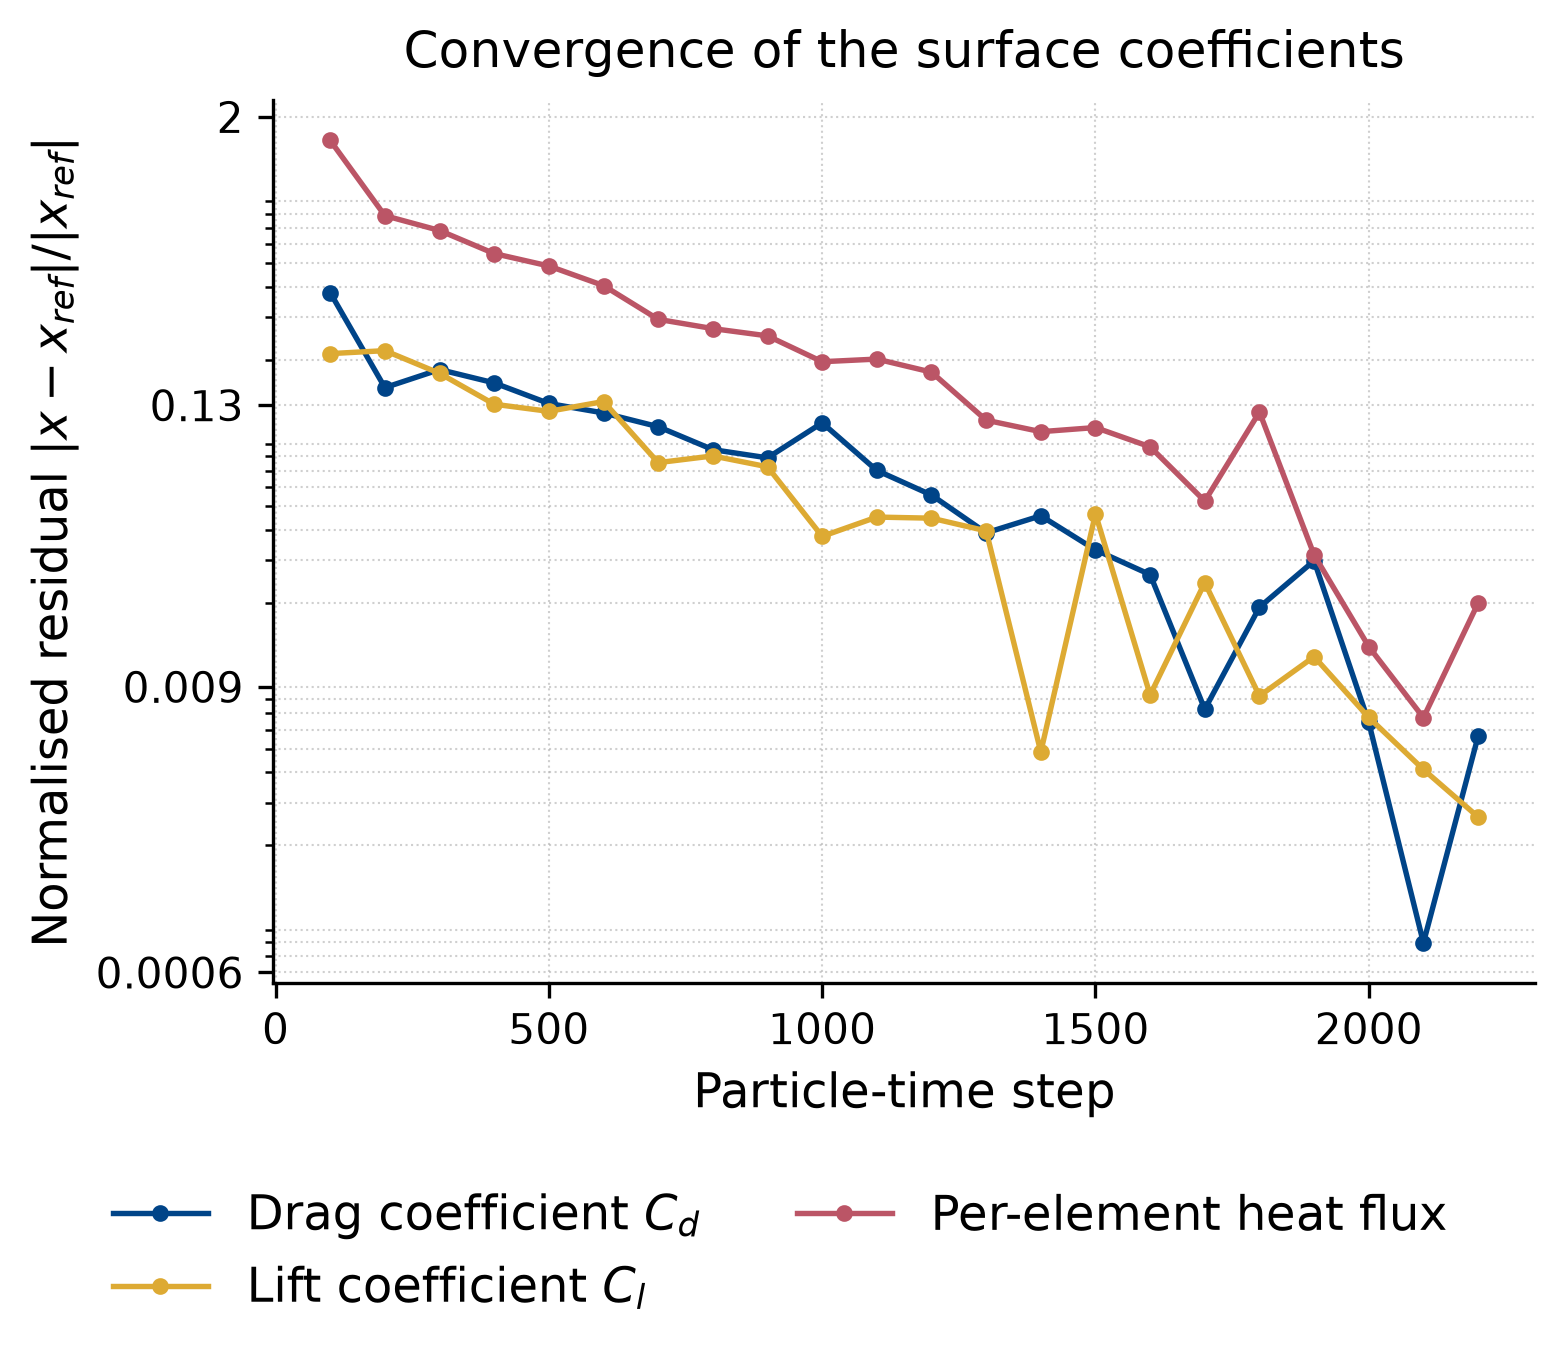
\includegraphics[width=0.9\columnwidth]{fignew_convergence_residuals.png}
\caption{Convergence of aerodynamic surface coefficients and per-element heat flux.}
\label{fig:conv}
\end{figure}

\section{Denoising}
DSMC data are noisy at the individual cell level. Kriging denoising recovers a smoother mean field while preserving the peak stagnation quantity. Figure~\ref{fig:krig} compares denoised and raw fields.

\begin{figure}[t]
\centering
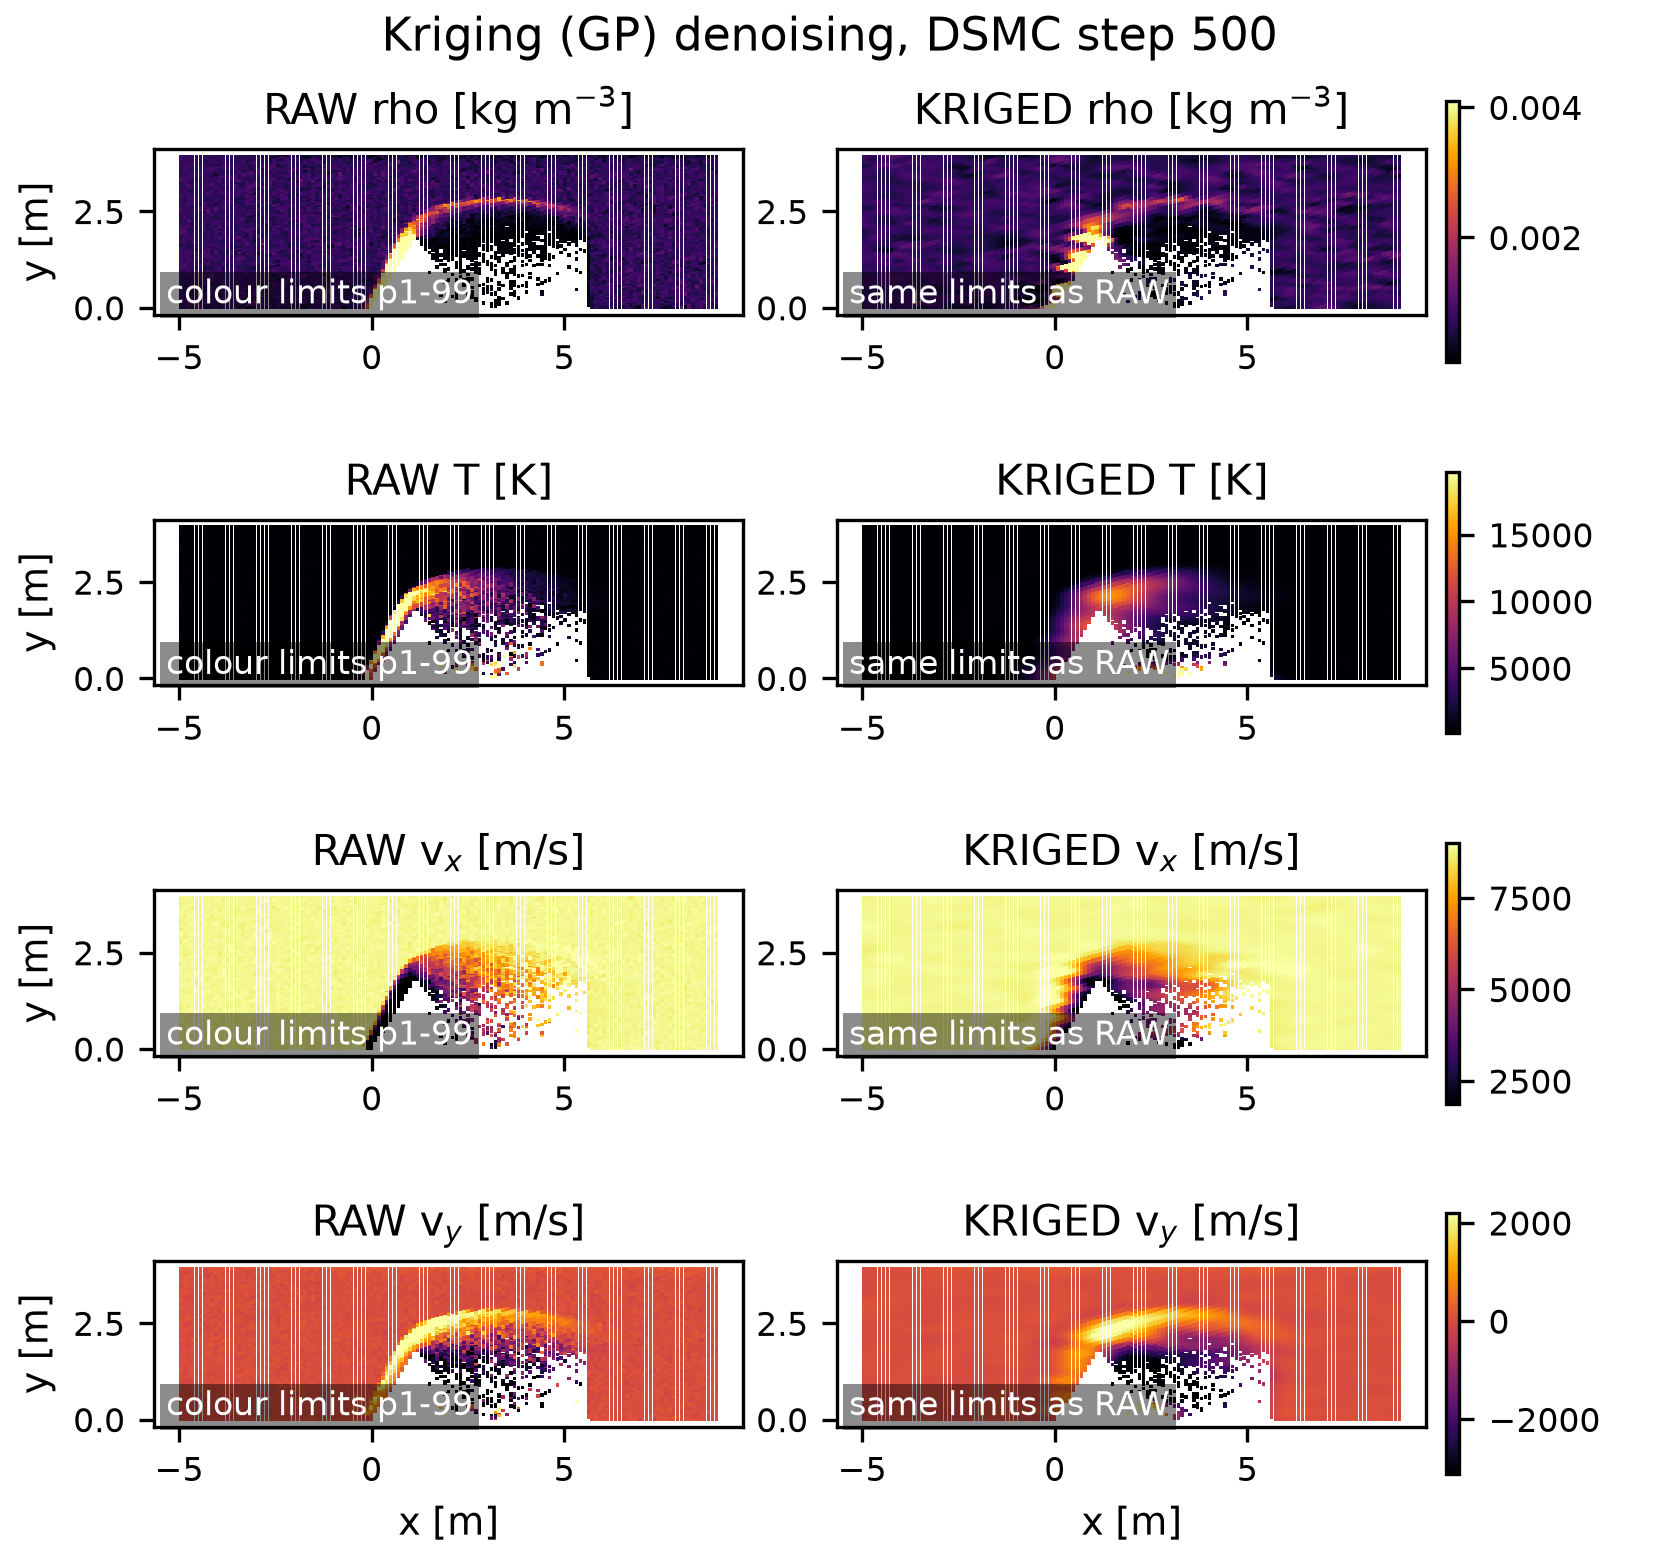
\includegraphics[width=0.9\columnwidth]{kriging_denoise.png}
\caption{Kriging denoising of the DSMC field.}
\label{fig:krig}
\end{figure}

\section{Capability and Limits}
Because the PINN relies on the continuum Navier-Stokes residual, its refined fields are valid only where the cell-scale Knudsen number stays inside the continuum band. The DSMC field map showed the slip band only across the shock interior, so the PINN cannot extend into the transitional regime. The refined fields are therefore restricted to the survivability comparison: whether the backface temperature of the material stack remains below its structural limit.

\noindent\textit{Novelty.} The contribution is the combination of an NS-residual PINN with Kriging denoising on DSMC samples for a HIAD, restricted to the continuum band, feeding a survivability assessment.\par\vspace{0.3em}
\section{Conclusion}
The PINN thread provides a differentiable, dense reconstruction of the aerothermal field from DSMC samples, with a composite loss built on the Navier-Stokes residual and Kriging denoising. It is validated only in the continuum band and feeds the survivability assessment. The pipeline is implemented inside the StellarOrion solver stack and is reproducible from CadQuery geometry forward.

\begin{sloppypar}\tolerance=9999 \emergencystretch=3em \raggedright
\noindent\textit{Limitations.} The PINN is restricted to the continuum band; it is not a substitute for DSMC in the slip or transitional regimes, and the reported backface value is taken from the companion TPS paper.\par\vspace{0.3em}
\noindent\textit{Reproducibility.} The architecture, weights and hyperparameter schedules are exported with the StellarOrion pipeline, and the DSMC input required to reproduce the PINN data term is the $2200$-particle-per-cell run described in the DSMC paper.\par\vspace{0.5em}
\noindent\textit{Future work.} Incorporate compressible turbulence and localized regions where slip effects matter.\par\vspace{0.3em}
\begin{thebibliography}{99}
\bibitem{raissi} M.~Raissi, P.~Perdikaris, and G.~E.~Karniadakis, ``Physics-Informed Neural Networks: A Deep Learning Framework for Solving Forward and Inverse Problems Involving Nonlinear PDEs,'' \emph{Journal of Computational Physics}, vol. 378, pp. 686--707, 2019.
\bibitem{baydin} A.~G.~Baydin et~al., ``Automatic Differentiation in Machine Learning,'' \emph{Journal of Machine Learning Research}, vol. 18, pp. 1--43, 2018.
\bibitem{kriging} C.~E.~Rasmussen and C.~K.~I.~Williams, \emph{Gaussian Processes for Machine Learning}, MIT Press, 2006.
\bibitem{bird} G.~A.~Bird, \emph{Molecular Gas Dynamics and the Direct Simulation Monte Carlo Method}, Oxford University Press, 1994.
\bibitem{sparka} SPARTA DSMC solver documentation, Sandia National Laboratories.
\bibitem{ref53} Zhu, J., Qiu, J., \& Shu, C. (2020). New developments of WENO schemes and their applications in computational fluid dynamics. Journal of Computational Physics, 401, 109009. https://doi.org/10.1016/j.jcp.2019.109009.
\bibitem{ref52} Zhang, R., Zhang, M., \& Shu, C. (2011). On the Order of Accuracy and Numerical Performance of Two Classes of Finite Volume WENO Schemes. Communications in Computational Physics, 9(3), 807-827. https://doi.org/10.4208/cicp.291109.080410s.
\bibitem{ref46} Sod, G. (1978). A survey of several finite difference methods for systems of nonlinear hyperbolic conservation laws. Journal of Computational Physics, 27(1), 1-31. https://doi.org/10.1016/0021-9991(78)90023-2.
\bibitem{ref41} Rusanov, V. (1962). The Calculation of the Interaction of Non-Stationary Shock Waves with Obstacles. USSR Computational Mathematics and Mathematical Physics, 1(2), 304-320. https://doi.org/10.1016/0041-5553(62)90062-9.
\bibitem{ref37} Plimpton, S., \& Gallis, M. (2014). SPARTA: A parallel DSMC code for rarefied gas dynamics. Journal of Computational Physics..
\bibitem{ref30} Liu, X., Osher, S., \& Chan, T. (1994). Weighted Essentially Non-Oscillatory Schemes. Journal of Computational Physics, 115(1), 200-212..
\bibitem{ref17} Harten, A., Engquist, B., Osher, S., \& Chakravarthy, S. (1987). Uniformly High Order Accurate Essentially Non-Oscillatory Schemes, III. Journal of Computational Physics, 71(2), 231-303..
\bibitem{ref342} A. Albee et al., Report on the loss of the mars polar lander and deep space 2 missions, 2000..
\bibitem{ref323} S. Koziel and X.-S. Yang, Computational optimization, methods and algorithms. Springer, 2011, vol. 356..
\bibitem{ref321} K. Deep, K. P. Singh, M. Kansal, and C. Mohan, A real coded genetic algorithm for solving integer and mixed integer optimization problems, Applied Mathematics and Computation, vol. 212, no. 2, pp. 505518, 2009. DOI: 10.1016/j.amc.2009.02.044..
\bibitem{ref319} S. Sivanandam and S. Deepa, Applications of genetic algorithms, Introduction to Genetic Algorithms, pp. 317402, 2008. DOI: 10.1007/978-3-540-73190-0\_10..
\bibitem{ref316} J. Kennedy and R. Eberhart, Particle swarm optimization, Proceedings of ICNN95 International Conference on Neural Networks, 1995. DOI: 10.1109/icnn.1995.488968..
\bibitem{ref295} B. M. Betsy, P. K. Mereena, R. M. Rincy, K. K. Vishnupriya, and D. Deepak, Design of thermal protection system for low ballistic coefficient ballute for ballistic earth re-entry, International Research Journal of Engineering and Technology (IRJET), vol. 7, no. 9, pp. 211230, Sep. 2020..
\bibitem{ref288} J. Moss, R. Wilmoth, J. Price, J. Moss, R. Wilmoth, and J. Price, DSMC simulations of blunt body flows for Mars entries - mars pathfinder and Mars microprobe capsules, 32nd Thermophysics Conference, 1997. DOI: 10.2514/6.1997-2508..
\bibitem{ref259} A. Diwakar and K. Bodi, Numerical and empirical studies of heat transfer in highenthalpy argonair mixtures, Journal of Thermophysics and Heat Transfer, vol. 36, no. 3, pp. 694706, 2022. DOI: 10.2514/1.t6311..
\bibitem{ref254} F. De Filippis and M. Serpico, Air high-enthalpy stagnation point heat flux calculation, Journal of Thermophysics and Heat Transfer, vol. 12, no. 4, pp. 608610, 1998. DOI: 10.2514/2.6386..
\bibitem{ref244} T. K. West and A. M. Brandis, Updated stagnation point aeroheating correlations for mars entry, 2018 Joint Thermophysics and Heat Transfer Conference, 2018. DOI: 10. 2514/6.2018-3767..
\bibitem{ref241} G. Benedetti, N. Viola, E. Minisci, A. Falchi, and M. Vasile, Low-fidelity modelling for aerodynamic characteristics of re-entry objects, Astrophysics and Space Science Proceedings, pp. 247264, 2018. DOI: 10.1007/978-3-319-69956-1\_15..
\bibitem{ref236} R. Wilmoth, R. Mitcheltree, J. Moss, R. Wilmoth, R. Mitcheltree, and J. Moss, Lowdensity aerodynamics of the stardust sample return capsule, 32nd Thermophysics Conference, 1997. DOI: 10.2514/6.1997-2510..
\bibitem{ref232} C. Cercignani and M. Lampis, Kinetic models for gas-surface interactions, Transport Theory and Statistical Physics, vol. 1, no. 2, 1971. DOI: 10.1080/00411457108231440..
\bibitem{ref228} L. A. Sinpetru et al., ADBSAT: Verification and validation of a novel panel method for quick aerodynamic analysis of satellites, Computer Physics Communications, vol. 275, p. 108 327, 2022. DOI: 10.1016/j.cpc.2022.108327..
\bibitem{ref217} L. A. Sinpetru, N. H. Crisp, D. Mostaza-Prieto, S. Livadiotti, and P. C. Roberts, ADBSAT: Methodology of A novel panel method tool for aerodynamic analysis of satellites, Computer Physics Communications, vol. 275, p. 108 326, 2022. DOI: 10.1016/j.cpc. 2022.108326..
\bibitem{ref215} G. Pezzella, P. Catalano, and A. Bourgoing, Computational flowfield analysis of a sample return capsule, 18th AIAA/3AF International Space Planes and Hypersonic Systems and Technologies Conference, 2012. DOI: 10.2514/6.2012-5818..
\bibitem{ref205} G. A. Bird, Definition of mean free path for real gases, Physics of Fluids, vol. 26, no. 11, p. 3222, 1983. DOI: 10.1063/1.864095..
\bibitem{ref180} J. R. Martins and J. T. Hwang, Review and unification of methods for computing derivatives of multidisciplinary computational models, AIAA Journal, vol. 51, no. 11, pp. 2582 2599, 2013. DOI: 10.2514/1.j052184..
\end{thebibliography}
\end{sloppypar}

\end{document}
